\documentclass[12pt,fleqn]{article}\usepackage{../common}
\begin{document}
Lineer Cebir - Ders 3

Onceki derslerde matris carpimi yaptik, bu derste bu islemin kurallarini
gorecegiz. Bu isi pek cok sekilde yapmanin yolu var ve hepsi onemli, ve
ayni sonucu veriyor.

Sonra matris tersi (inverse) konusuna girecegiz, orada bir suru kavram var,
ve cok onemli. 

Iki matrisi carpma teknigiyle baslayalim. 

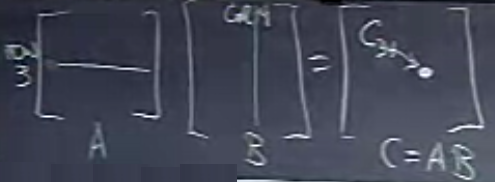
\includegraphics[height=3cm]{3_01.png}

Bu carpimi elle yaparken bazen soldaki matrisin uzerinde sol isaret
parmagi, sagdakinde sag isaret parmagi konulur, ve sol el soldan-saga, sag
el yukaridan-asagi hareket ettirilir, ve parmaklarin uzerinde olan hucreler
birbiri ile carpilir, sonra bu carpimlar toplanir. Ustte soldaki matrisin
3. satiri, sagdaki matrisin 4. kolonu baz alinmis, bu carpim ve toplama
sonucu $C$'nin 3. satir ve 4. kolonundaki degeri elde ederiz. Bu degere
$c_{34}$ diyelim,

$$ 
\left[\begin{array}{rrrr}
\\
\\
a_{31} & a_{32} & \dots \\
\\
\\
\end{array}\right]
\left[\begin{array}{rrrrr}
& & b_{14} & & \\
& & b_{24} & & \\
& &  & & \\
& &  & & \\
& &  & & 
\end{array}\right] 
=
\left[\begin{array}{rrrrr}
& &  & & \\
& &  & & \\
& & c_{34} & & \\
& &  & & \\
& &  & & 
\end{array}\right]
$$

$$ c_{34} = \textrm{ 3. satir } \times \textrm{ 4. kolon } $$

diyebiliriz, ve cebirsel olarak

$$ = a_{31}b_{14} + a_{32}b_{24} + ... $$

Eger toplama operatoru kullanarak daha temiz yazmak gerekirse,

$$ c_{34} = \sum_{k=1}^{n} a_{3k}b_{k4} $$
ki $n$ satir sayisi $n$'dir. 

Bu carpimi tabii her zaman gerceklestiremeyiz. Carpimin olmasi icin matris
boyutlarinin uyumlu olmasi gerekir (illa kare matris olmasi da gerekmez,
ama uyumluluk gerekir). Ustteki carpimin nasil gerceklestigine bakarsak bu
uyumu gormeye baslariz herhalde, soldaki matrisin satiri sagdakinin kolonu
carpiliyorsa bu satir ve kolon buyukluklerinin esit olmasi gerekir. Diyelim
ki $m$ satir $n$ kolon iceren $A$ matrisi $m \times n$ boyutlarinda ise, o
zaman bu matris sadece $n \times p$ boyutlarindaki bir $B$ matrisi ile
carpilabilir, ve sonuc $m \times p$ boyutlarinda yeni bir matris
olur. Yeni matrisin boyutlari $A$'nin satir sayisi $B$'nin kolon sayisina
esittir. 

Matris carpimina kolon bazli bakabilir miyiz? Evet. Daha once ogrendigimiz
kolonla matris carpimi fikrini kullanmak yeterli, mesela alttaki durumda

$$ 
\underbrace{
\left[\begin{array}{rr}
\dots & \dots   \\
\dots & \dots   \\
\dots & \dots 
\end{array}\right]
}_{A m \times n}
\underbrace{
\left[\begin{array}{rr}
\uparrow &  \dots\\
&  \dots\\
\downarrow & \dots 
\end{array}\right] 
}_{B, n \times p}
=
\underbrace{
\left[\begin{array}{rr}
\uparrow &  \dots \\
&  \dots \\
\downarrow & \dots
\end{array}\right] 
}_{C, m \times p}
$$

$A$'nin {\em tamaminin} $B$'nin en sol kolonu ile carpilmasi bize $C$'nin
en sol kolonunu verecektir. Dikkat, bu islemde $B$'nin diger kolonlari
hicbir sekilde isleme dahil olmazlar. Yine eger yine $A$'nin {\em tamami}
ile bu sefer ikinci kolonu carparsak $C$'nin ikinci kolonunu elde ederiz,
vs.

$$ 
\underbrace{
\left[\begin{array}{rr}
\dots & \dots   \\
\dots & \dots   \\
\dots & \dots 
\end{array}\right]
}_{A m \times n}
\underbrace{
\left[\begin{array}{rr}
\dots & \uparrow \\
& \\
\dots & \downarrow
\end{array}\right] 
}_{B, n \times p}
=
\underbrace{
\left[\begin{array}{rr}
\dots & \uparrow \\
& \\
\dots & \downarrow
\end{array}\right] 
}_{C, m \times p}
$$

O zaman su ifadeyi kullanabiliriz: ``$C$'nin kolonlari $A$'nin kolonlarinin
bir kombinasyonudur''. Bu ifade daha onceki kolon bakisimiz ile
uyumlu. Daha once kolonlarin kombine edilerek yeni bir kolon elde
edildigini gorduk, bu fikri sadece $B$ uzerinde, tekrar tekrar, her $B$
kolonu ile ayri ayri uyguluyoruz, ve sonuc olarak $C$'nin ayri ayri
kolonlarini elde ediyoruz.

Satir Bakisi

$$ 
\underbrace{
\left[\begin{array}{rr}
\leftarrow  & \rightarrow  \\
\dots & \dots \\
\dots & \dots 
\end{array}\right]
}_{A m \times n}
\underbrace{
\left[\begin{array}{rr}
\dots & \dots \\
\dots & \dots \\
\dots & \dots
\end{array}\right] 
}_{B, n \times p}
=
\underbrace{
\left[\begin{array}{rr}
\leftarrow  & \rightarrow  \\
\dots & \dots  \\
\dots & \dots 
\end{array}\right] 
}_{C, m \times p}
$$

Ayni carpimi satirsal olarak dusunelim, tekrar daha once ogrendigimiz satir
bakisini ayri ayri satirlar olarak kullaniyoruz. $A$'nin tek bir satiri
$B$'nin tamamini, tum satirlarini kombine ediyor ve bu sekilde $C$'nin
tekabul eden satirini elde ediyoruz. 

Peki 4. yol nedir? Simdiye kadar gorduklerimiz satir ve kolon noktasal
carpimi (her $C$ hucresi icin), $A$ kolon kombinasyonu, $B$ satir
kombinasyonu. Ya peki $A$'nin kolonunu alip $B$'nin satiriyla carpsak ne
olur? Boyut olarak bu neye benzerdi? $A$'dan tek kolon alinca boyut $m
\times 1$. $B$'den satir alinca boyut $1 \times p$. Carpinca sonuc bir
matris olmaz mi? Evet, boyutu $m \times p$ boyutunda bir matris ortaya
cikar. Bunu iki vektorun carpimindan elde ettik! Ufak bir ornekte gorelim, 

$$ 
\left[\begin{array}{r}
2 \\ 3 \\ 4
\end{array}\right]
\left[\begin{array}{rr}
1 & 6
\end{array}\right]
=
\left[\begin{array}{rr}
2 & 12 \\
3 & 18 \\
4 & 24
\end{array}\right]
 $$

 Sagdaki matris cok ozel bir matristir; oncelikle $C$'nin kolonlari mesela
 $A$'nin (su anda bir vektor) katlaridir aslinda. Peki satirlar?  $C$'nin
 satirlari ayni zamanda $B$ nin satirlarinin da katlaridir! O zaman sunu
 soyleyebiliriz. 4. yol $k=1,..,n$ icin $A$'nin $k$'inci kolonu ile
 $k$'inci satirinin carpiminin toplamidir. Yani alttaki gibi ornekte
 gostermek gerekirse, 

$$ 
\left[\begin{array}{rr}
2 & 7 \\
3 & 8 \\
4 & 9
\end{array}\right]
\left[\begin{array}{rr}
1 & 6 \\
0 & 0
\end{array}\right]
=
\left[\begin{array}{r}
2 \\ 3\\ 4
\end{array}\right]
\left[\begin{array}{rr}
1 & 6
\end{array}\right] 
+
\left[\begin{array}{r}
7 \\ 8\\ 9
\end{array}\right]
\left[\begin{array}{rr}
0 & 0
\end{array}\right] 
 $$

Esitligin saginda her toplamda ayri birer matris var. Yani her carpimdan
bir matris elde ediyoruz, sonra bu matrisleri ust uste koyarak
topluyoruz. Bu yaklasim ayri ayri kolonlari hesaplayip onlari yanyana
istiflemekten farkli, 4. yolda $m \times p$ boyutlu bir matrisi surekli
elde ediyoruz, sonra bu matrisleri topluyoruz. 

Eger iki ustteki ornekteki $C$'nin satirlarini vektor olarak cizseydim,
onlarin hepsinin ayni yone isaret ettigini gorurdum; ust uste binmis farkli
boyutlarinda vektorler olarak gozukuyorlerdi yani. Kolonlari cizsem, yine
ayni sekilde olurlardi. Simdi bir ifade kullanacagim, ki anlami dersin
ilerisinde daha acik hale gelecek, ``$C$'nin satir uzayi da, kolon uzayi da
tek bir cizgidir (ayri cizgiler tabii)''.

Blok Teknigi

Aslinda matrisleri parcalara bolup carpimi o parcalar uzerinde yapmak ta
mumkundur. 

Mesela $A$'yi ve $B$'yi dort parcaya bolebilirim, ki $A$ mesela $10 \times
10$ boyutlarinda olabilir, o zaman carpim sonucunun sol ust kosesi ne olur?
Alttaki gibi olur,

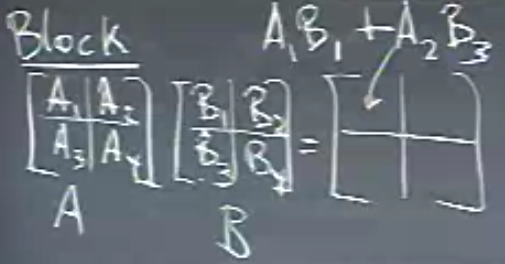
\includegraphics[height=4cm]{3_02.png}

Yani bloklari sanki tekil hucreymis gibi gorup bildigimiz carpim numarasini
uygulayabiliyoruz. 

Evet bugunluk matris carpimi konusunu bitirdik. Artik matris tersi alma
konusuna gelebiliriz. 

Matris Tersi (Inverses)

Matris tersi $A^{-1}$ mesela bir $A$ matrisi icin, eger var ise, oyle bir
matristir ki $A$ ile carpilinca birim matrisi verir. Yani

$$ A^{-1} A = I $$

Tabii bu durum biraz daha detaylandirilabilir; mesela ustteki matris tersi
soldan ters (left inverse) olarak bilinir, ama kare matrisler icin soldan,
sagdan hepsi aynidir, yani kare durum icin 

$$ AA^{-1} = I $$

ifadesi de dogrudur. Bunu ispat etmek pek kolay degildir bu arada. Neyse,
karesel degil dikdortgensel matris olsaydi o zaman sol ters sag terse esit
olmazdi; zaten boyut acidan bu esitlik imkansiz olurdu. Karesel acidan
boyutlar da uyumlu. 

Onemli sorular matris tersi ne zaman mevcuttur, ve mevcut ise nasil
bulunur. 

Tersi alinabilen matrisler ayni zamanda tekil olmayan (non-singular)
matrislerdir. Simdi tekil olan ve tersi olmayan duruma bakalim. Ufak ornek, 

$$ 
A = 
\left[\begin{array}{rr}
1 & 3 \\ 2 & 6
\end{array}\right]
 $$

Bu matrisin niye tersi yoktur? Bu soruya degisik sekillerde cevap
verilebilir. Eger determinantlari gormus olsaydik derdik ki ``determinanti
hesaplayinca sifir sonuc gelir''. Baska bir sebep? 

Diyelim ki $A$ bir baska matrisle carpilinca birim matris sonucunu
verdi. Bu baska matris nedir? Eger ters yoksa, bu mumkun olamaz. Niye?
Simdi kolon bakisini dusunelim, eger $A$'yi bir baska matris ile
carpiyorsam ters olmayan durumda kolonlar birbirinin katidir. Peki
birbirinin kati olan kolonlarin kombinasyonu ile birim matris elde edebilir
miyim? Mumkun degil. Cunku birim matrisin kolonlarinda 1 ve 0 degerleri
var, ve ustteki durumda katlari ekleyerek cikartarak, vs bu degerlere
ulasamam. 

Bir diger bakis acisi: $Ax = 0$ denklemini tatmin edecek bir $x$ vektoru
bulabilir miyim? Matris formunda yazarsam, 

$$ 
\left[\begin{array}{rr}
1 & 3 \\ 2 & 6
\end{array}\right]
\left[\begin{array}{r}
\dots \\ \dots
\end{array}\right]
=
\left[\begin{array}{r}
0 \\ 0
\end{array}\right]
 $$

Noktali yerlere ne gelmeli? Ne gelebilir? 

$$ 
\left[\begin{array}{rr}
1 & 3 \\ 2 & 6
\end{array}\right]
\left[\begin{array}{r}
3 \\ -1
\end{array}\right]
=
\left[\begin{array}{r}
0 \\ 0
\end{array}\right]
 $$
 
Simdi bir zihin egzersizi: Eger $A$'nin tersi olsaydi, her iki tarafi
matris tersiyle carpardim,

$$A^{-1}Ax = A^{-1} 0$$

$$x = 0$$

sonucunu elde ederdim. Yani $x=0$ olmasi gerekirdi. Fakat $x \ne 0$, biraz
once ustte bunu bulduk. Burada bir cakisma var (contradiction), demek ki
baslangic hipotezi yanlistir; $A$'nin tersi yoktur. 

Tersi olan bir matris alalim. Bosluga ne gelmeli?

$$ 
\underbrace{
\left[\begin{array}{rrr}
1 & 3 \\
2 & 7
\end{array}\right]
}_{A}
\underbrace{
\left[\begin{array}{rrr}
 &  \\
 & 
\end{array}\right]
}_{A^{-1}}
=
\underbrace{
\left[\begin{array}{rrr}
1 & 0 \\
0 & 1
\end{array}\right]
}_{I}
 $$
Kolonsal olarak dusunelim, 


$$ 
\underbrace{
\left[\begin{array}{rrr}
1 & 3 \\
2 & 7
\end{array}\right]
}_{A}
\underbrace{
\left[\begin{array}{rrr}
a &  \\
b & 
\end{array}\right]
}_{A^{-1}}
=
\underbrace{
\left[\begin{array}{rrr}
1 &  \\
0 & 
\end{array}\right]
}_{I}
 $$

Yani tersin ilk kolonuna oyle $a,b$ degerleri bulalim ki bu kolon $A$'yi
carpinca (kolonlarini kombine edince) sonuc $\left[\begin{array}{rr}1 &
    0\end{array}\right]^T$ olsun. 

Ayni sekilde ikinci kolon icin ama bu sefer sonuc $\left[\begin{array}{rr}0 &
 1\end{array}\right]^T$ olsun. 


$$ 
\underbrace{
\left[\begin{array}{rrr}
1 & 3 \\
2 & 7
\end{array}\right]
}_{A}
\underbrace{
\left[\begin{array}{rrr}
a & c \\
b & d
\end{array}\right]
}_{A^{-1}}
=
\underbrace{
\left[\begin{array}{rrr}
1 & 0 \\
0 & 1
\end{array}\right]
}_{I}
 $$

Belki de soyle soylemek lazim; burada ayni anda iki denklem sistemi
cozuyor gibiyiz. Bu baglamda Gauss-Jordan'in fikri sudur; her iki denklemi
ayni anda coz. Denklemler sunlardir

$$ 
\left[\begin{array}{rrr}
1 & 3 \\
2 & 7
\end{array}\right]
\left[\begin{array}{r}
a  \\
b 
\end{array}\right]
=
\left[\begin{array}{rrr}
1  \\
0
\end{array}\right]
 $$

$$ 
\left[\begin{array}{rrr}
1 & 3 \\
2 & 7
\end{array}\right]
\left[\begin{array}{r}
c  \\
d 
\end{array}\right]
=
\left[\begin{array}{rrr}
0  \\
1
\end{array}\right]
 $$

Gauss ile Jordan bu konu hakkinda konusuyorlarmis, Jordan Gauss'a
``bunlarin ikisini niye ayni anda cozmuyorsun?'' demis. Hikaye boyle! Bunun
icin Jordan'in fikri eklemlemeyi genisletmektir. Daha once gordugumuz gibi,
denklem cozmek demek, eklemlenmis (augmented) matrisi cozmek demektir,
1. denklem icin 

$$ 
\left[\begin{array}{rr|r}
1 & 3 & 1\\
2 & 7 & 0
\end{array}\right]
 $$

cozulurdu mesela. Iki denklem icin fikir 2. sonucu da eklemlenmis kisma
koymak, yani 
        
$$ 
\left[\begin{array}{rr|rr}
1 & 3 & 1 & 0\\
2 & 7 & 0 & 1
\end{array}\right]
 $$

sistemini cozmek. Ustteki sistem cozulunce sonuc matris tersi olacaktir!
Cunku eklemlenmis kisima dikkat edersek, o kisim aslinda bir birim
matrisidir. Simdi eliminasyona baslariz, mesela 1. satiri 2 ile carpip
2. satirdan cikartmak yani,

        
$$ 
\left[\begin{array}{rr|rr}
1 & 3 & 1 & 0\\
0 & 1 & -2 & 1
\end{array}\right]
 $$

elde ederiz. Ustteki sol matris ust ucgensel. Bu noktada Gauss ``is
tamamdir'' demis, fakat Jordan devam et diyor. Simdi en ust satirdaki 3
sayisini elimine et. O zaman alttaki satiri 3 ile carpip 1. satirdan
cikartiriz,

$$ 
\left[\begin{array}{rr|rr}
1 & 0 & 7 & -3\\
0 & 1 & -2 & 1
\end{array}\right]
 $$

Boylece sol kisimda birim matris edildi. Ve tanim itibariyle sag kisimda
ise $A^{-1}$ elde etmis oldum. Peki bu nasil oldu? Elimizde bir
$\left[\begin{array}{r|r}A & I\end{array}\right]$ var, ve onda eliminasyon yapiyorum, yani onu bir suru $E$ ile ardarda 
carpiyorum, ya da tek nihai bir $E$ ile carpiyorum. 

$$ E \left[\begin{array}{rr}A & I\end{array}\right] = 
\left[\begin{array}{rr}I & ?\end{array}\right]
$$

Eger $EA = I$ elde edebiliyorsam, $E$ oyle bir seydir ki $A$ ile carpinca
bana $I$ vermektedir. Bu ``sey'' o zaman matris tersinden baska bir sey
olamaz, yani $E = A^{-1}$. Devam edersek,

$$ E \left[\begin{array}{rr}A & I\end{array}\right] = 
\left[\begin{array}{rr}EA & EI\end{array}\right] =
\left[\begin{array}{rr}I & EI\end{array}\right] =
\left[\begin{array}{rr}I & E\end{array}\right] =
\left[\begin{array}{rr}I & A^{-1}\end{array}\right]
$$

$E$ birim matrisi ile carpildi. Demek ki sonuc matrisinin sag kisminda
gorulen matris $E$'dir, yani matris tersidir.


\end{document}
